\documentclass[
  aspectratio=169,
]{beamer}

\usepackage[english]{babel}
\usepackage[utf8]{inputenc}
\usepackage[T1]{fontenc}
\usepackage{amsmath,amssymb,amsfonts}
\usepackage{booktabs}
\usepackage{array}
\usepackage{tabularx}
\usepackage{graphicx}
\usepackage{csquotes}

\usetheme[
  workplace=arch,
]{MU}

\title{Automated Document Layout Analysis and Hierarchical Transcription for Historical Indic Manuscripts}
\subtitle{A Geometry-First Formulation with Structural Segmentation and Morphological Decomposition}
\author{Dakshan Karthic}
\institute{Department of Computer Science and Engineering}
\date{}
\subject{Document Image Processing and Pattern Recognition}
\keywords{Document Layout Analysis, Optical Character Recognition, Devanagari Script, Morphological Image Processing, Semantic Segmentation, PAGE-XML}

% Clean Header: Remove Top Navigation Bar (Section / Subsection Text)
\setbeamertemplate{headline}{}

% Clean Footline: Slide Number Only (Author & Title Text Removed)
\setbeamertemplate{footline}{%
  \hfill\usebeamercolor[fg]{page number in head/foot}%
  \usebeamerfont{author in head/foot}\insertframenumber{} / \inserttotalframenumber\hspace*{1.5em}\vspace*{0.3cm}%
}

\begin{document}

% ─────────────────────────────────────────────────────────────
% FRAME 1: Title Frame
% ─────────────────────────────────────────────────────────────
\begin{frame}[plain]
\maketitle
\end{frame}

% ─────────────────────────────────────────────────────────────
% FRAME 2: Challenges Faced in Indic Manuscripts
% ─────────────────────────────────────────────────────────────
\section{Introduction and Problem Formulation}
\subsection{Physical and Orthographic Challenges}

\begin{frame}{Physical and Orthographic Challenges in Indic Manuscripts}{Continuous Headlines, Substrate Degradation, and Binder Punch Holes}
\centering
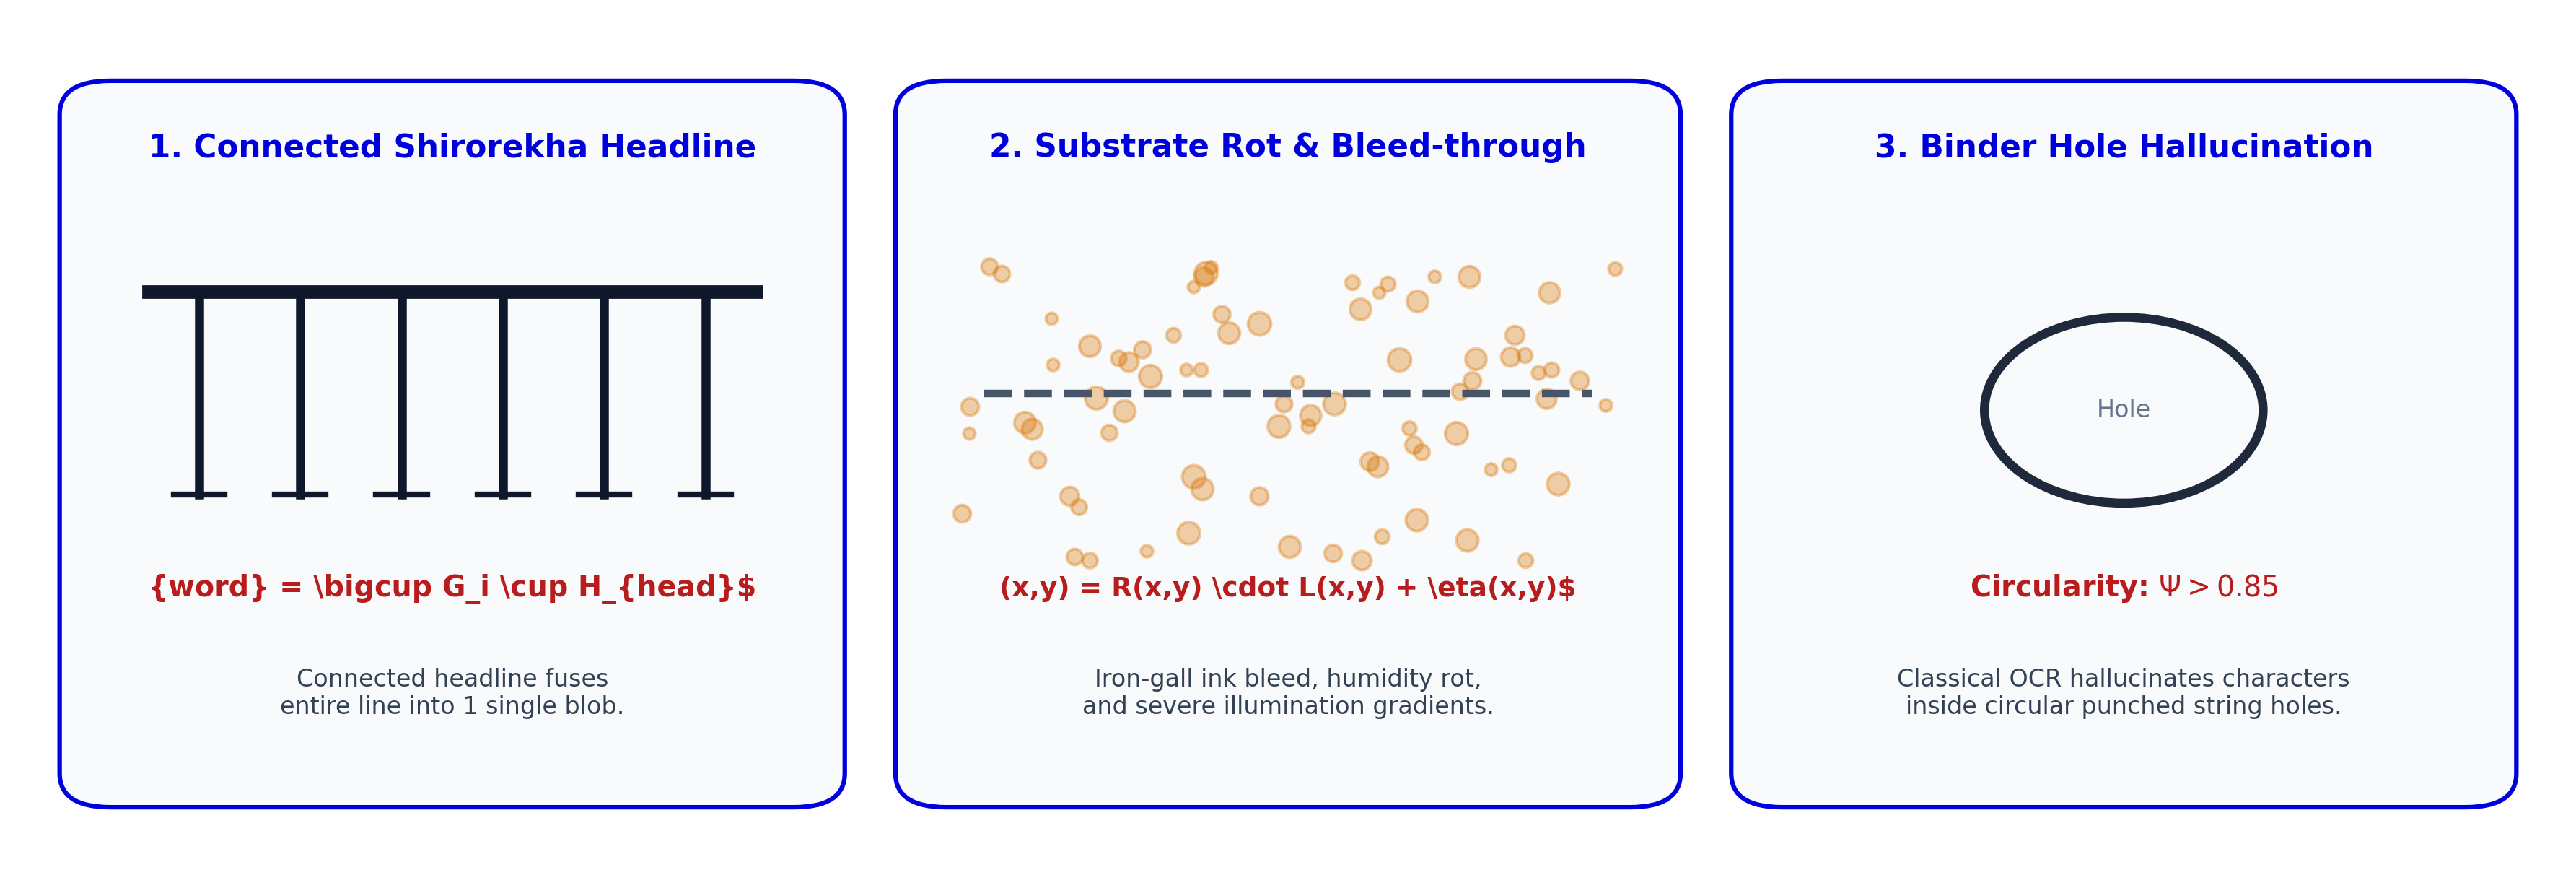
\includegraphics[width=0.92\textwidth,height=0.38\textheight,keepaspectratio]{shirorekha_challenge_demo.png}
\vspace{0.15cm}
\begin{columns}
  \begin{column}{0.48\textwidth}
    \begin{block}{1. Continuous Headline (\textit{Shirorekha})}
      Devanagari characters are fused along the top horizontal stroke:
      \[
        \mathcal{S}_{\text{word}} = \bigcup_{i=1}^{M} \mathcal{G}_i \cup \mathcal{H}_{\text{shirorekha}}
      \]
      Classical connected components fail by merging entire lines.
    \end{block}
  \end{column}
  \begin{column}{0.48\textwidth}
    \begin{block}{2. Substrate Decay \& Binder Holes}
      Illumination gradients, iron-gall bleed, and circular holes:
      \[
        I(x,y) = R(x,y) \cdot L(x,y) + \eta(x,y), \quad \Psi > 0.85
      \]
      Optical degradation causes frequent character hallucinations.
    \end{block}
  \end{column}
\end{columns}
\end{frame}

% ─────────────────────────────────────────────────────────────
% FRAME 3: Mathematical Problem Formulation
% ─────────────────────────────────────────────────────────────
\begin{frame}{Mathematical Problem Formulation}{Hierarchical Document Layout Representation}
\begin{block}{Objective Definition (PRImA PAGE-XML 2013 Framework)}
Given raw digital capture $I \in \mathbb{R}^{H \times W \times 3}$, determine hierarchical decomposition $\mathcal{T}$:
\[
  \mathcal{T} = \left\{ \mathcal{R}_{\text{frame}}, \{\mathcal{R}_{\text{text}}^{(k)}\}_{k=1}^{K}, \{\mathcal{R}_{\text{illus}}^{(m)}\}_{m=1}^{M}, \{\mathcal{R}_{\text{damage}}^{(d)}\}_{d=1}^{D}, \{\mathcal{L}_{j}\}_{j=1}^{J}, \{\mathcal{W}_{j,p}\}, \{\mathcal{G}_{j,p,q}\} \right\}
\]
\end{block}
\begin{itemize}
  \item \textbf{Region Boundaries:} Represented as closed planar polygons $\mathcal{P} = \{(x_1, y_1), \dots, (x_V, y_V)\}$.
  \item \textbf{Reading Order Continuity:} Ordered column permutation $\mathcal{C}_1 \prec \mathcal{C}_2 \prec \dots \prec \mathcal{C}_C$.
  \item \textbf{Mathematical Continuity:} Every stage output directly feeds the subsequent stage's input.
\end{itemize}
\end{frame}

% ─────────────────────────────────────────────────────────────
% FRAME 4: Proposed 3-Stage System Flowchart
% ─────────────────────────────────────────────────────────────
\section{Methodology}
\subsection{System Architecture and Pipeline Flowchart}

\begin{frame}{Proposed 3-Stage End-to-End System Architecture}{Continuous Pipeline from Raw Capture to Granular PAGE-XML Hierarchy}
\centering
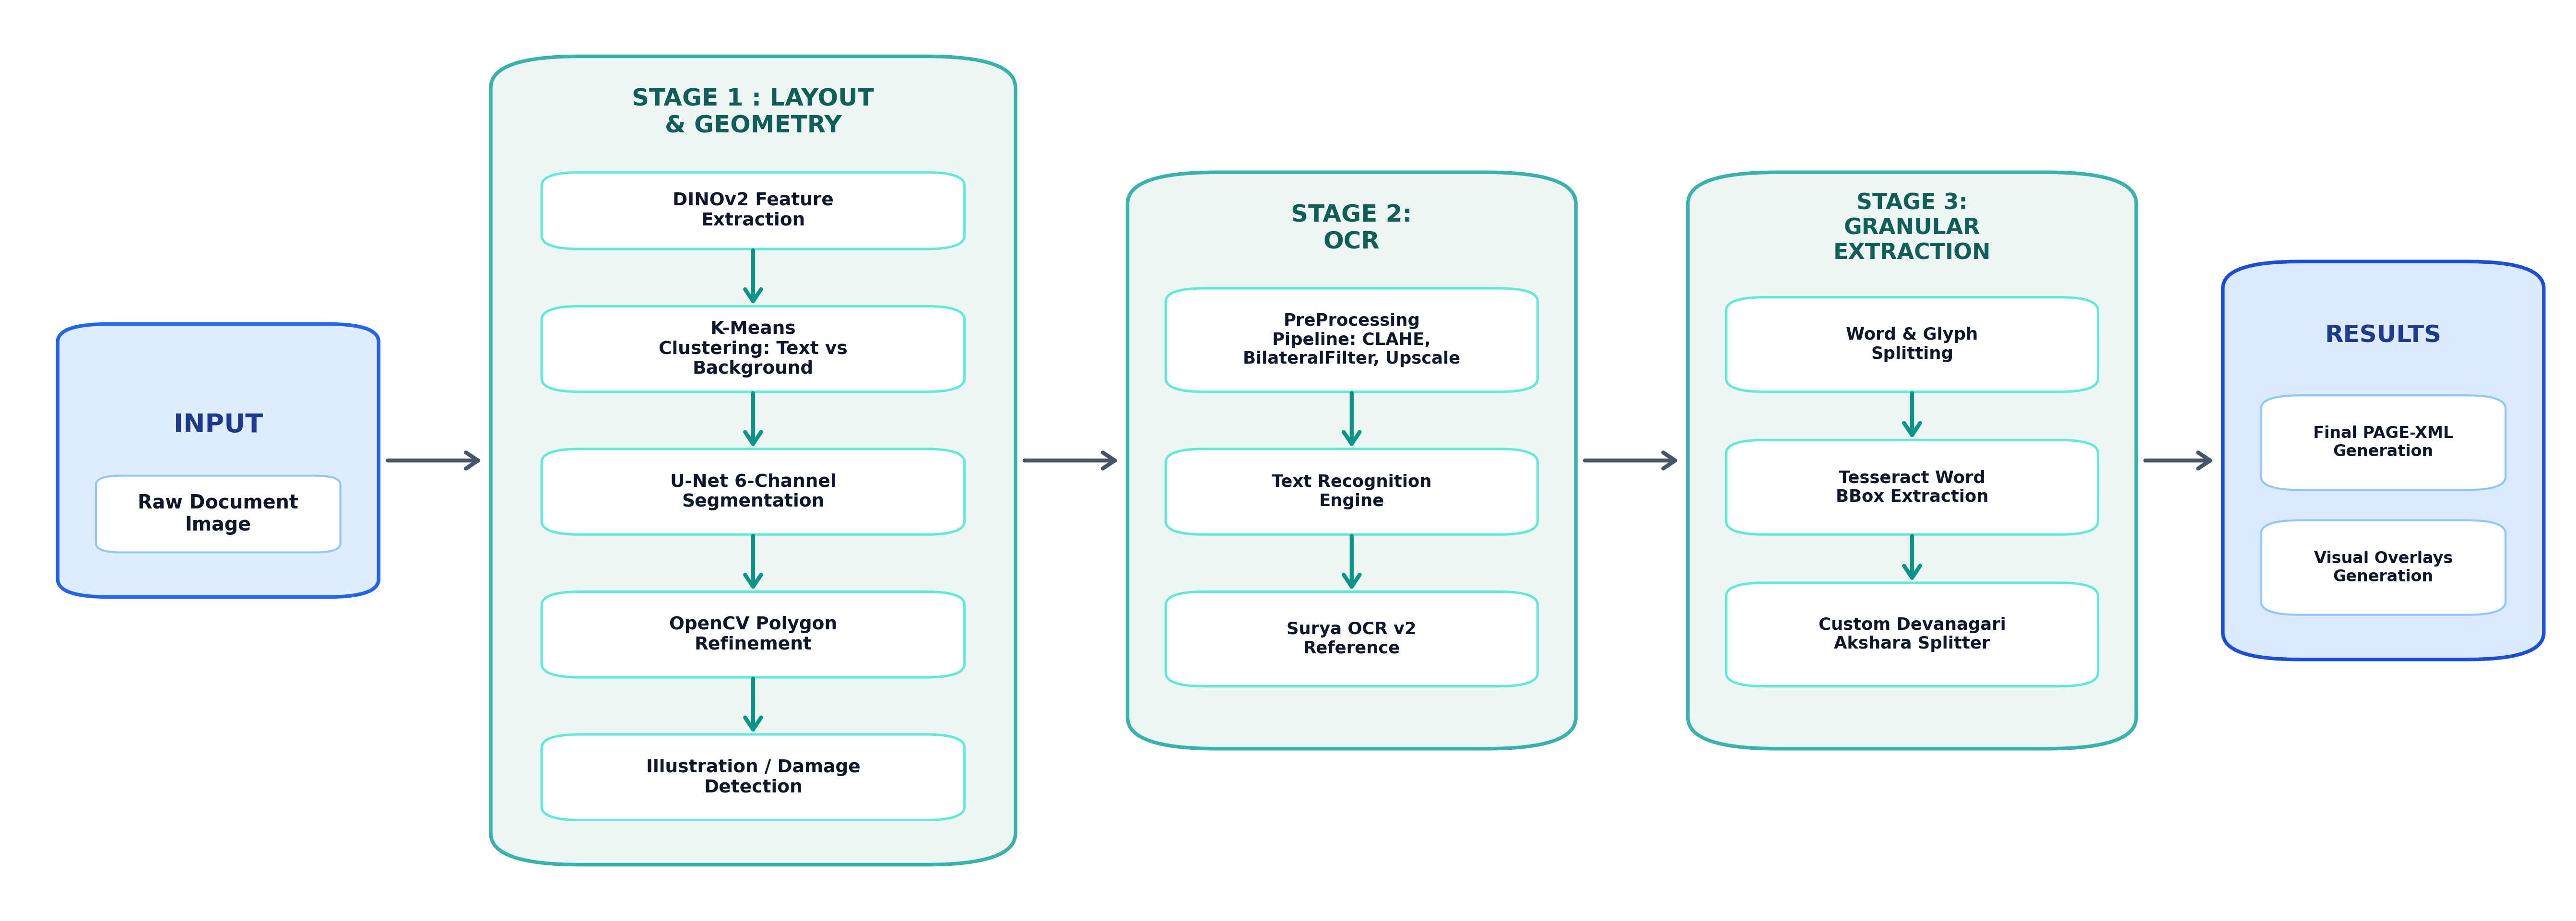
\includegraphics[width=\textwidth,height=0.72\textheight,keepaspectratio]{pipeline_flowchart_white.png}
\end{frame}

% ─────────────────────────────────────────────────────────────
% FRAME 5: Image Preprocessing & Adaptive Binarization
% ─────────────────────────────────────────────────────────────
\subsection{Stage 1: Layout Detection and Geometry}

\begin{frame}{Image Preprocessing and Adaptive Binarization}{Local Illumination Compensation}
\begin{block}{Adaptive Gaussian Thresholding: $I(x,y) \rightarrow B(x,y)$}
Foreground ink strokes are separated from non-uniform background substrates using local Gaussian statistics:
\[
  B(x,y) = \begin{cases} 
    1 & \text{if } I_{\text{gray}}(x,y) < \mu_G(x,y) - C \\
    0 & \text{otherwise}
  \end{cases}, \quad \mu_G(x,y) = (I_{\text{gray}} * G_\sigma)(x,y)
\]
Parameter configuration: local window radius $r=25$, constant subtraction $C=5$.
\end{block}
\begin{block}{Morphological Filtering: $B(x,y) \rightarrow B_{\text{clean}}(x,y)$}
Isolated substrate fiber noise is suppressed via morphological opening with structuring element $\mathcal{E}_{3\times 3}$:
\[
  B_{\text{clean}} = (B \ominus \mathcal{E}_{3\times 3}) \oplus \mathcal{E}_{3\times 3}
\]
\end{block}
\end{frame}

% ─────────────────────────────────────────────────────────────
% FRAME 6: Stage 1: DINOv2 Feature Geometry & Self-Attention
% ─────────────────────────────────────────────────────────────
\begin{frame}{Stage 1: Foundation Vision Transformer (DINOv2)}{Patch Embedding, Multi-Head Self-Attention, and Zero-Shot Manifolds}
\begin{block}{Patch Discretization \& Position Encoding: $I \rightarrow \mathbf{x}_0$}
Model: \texttt{DINOv2-ViT-B/14} ($D = 768, P = 14$). Image dimensions aligned to patch multiples ($N = \frac{H'}{14} \times \frac{W'}{14}$):
\[
  \mathbf{x}_0 = \left[ \mathbf{x}_{\text{cls}}; \, \mathbf{x}_p^1 \mathbf{E}; \, \dots; \, \mathbf{x}_p^N \mathbf{E} \right] + \mathbf{E}_{\text{pos}}, \quad \mathbf{E} \in \mathbb{R}^{588 \times 768}, \quad \mathbf{E}_{\text{pos}} \in \mathbb{R}^{(N+1) \times 768}
\]
\end{block}
\begin{block}{Multi-Head Self-Attention (MHSA) Affinity Matrix: $\mathbf{x}_0 \rightarrow \mathbf{Z}$}
Pairwise spatial attention across $h=12$ heads ($d_k = 64$) extracting intrinsic stroke geometry:
\[
  \text{Attention}(\mathbf{Q}, \mathbf{K}, \mathbf{V}) = \text{softmax}\left( \frac{\mathbf{Q} \mathbf{K}^T}{\sqrt{d_k}} \right) \mathbf{V}, \quad A_{ij} = \frac{\mathbf{z}_i \cdot \mathbf{z}_j}{\|\mathbf{z}_i\| \|\mathbf{z}_j\|} = \cos(\theta_{ij})
\]
\end{block}
\end{frame}

% ─────────────────────────────────────────────────────────────
% FRAME 7: Stage 1: Substrate-Adaptive Manifold Clustering
% ─────────────────────────────────────────────────────────────
\begin{frame}{Stage 1: Substrate-Adaptive Manifold Clustering}{Border-Invariant Feature Partitioning}
\begin{block}{Substrate Classification Metric: $I_{\text{gray}} \rightarrow \bar{L}_{\text{border}}$}
Boundary band luminance $\bar{L}_{\text{border}}$ distinguishes light paper from dark palm-leaf substrates:
\[
  \bar{L}_{\text{border}} = \frac{1}{|\mathcal{B}|} \sum_{(x,y) \in \mathcal{B}} I_{\text{gray}}(x,y), \quad \mathcal{B} = \text{Image Boundary Band}
\]
\end{block}
\begin{enumerate}
  \item \textbf{Case $\bar{L}_{\text{border}} > 200$ (Printed Paper Substrate, $k=2$):}
  Binary K-Means clustering on token embeddings $\mathbf{z}_i$:
  \[
    \mathcal{J}_{\text{paper}} = \sum_{i=1}^N \min_{j \in \{0,1\}} \|\mathbf{z}_i - \mathbf{c}_j\|^2
  \]
  \item \textbf{Case $\bar{L}_{\text{border}} \le 200$ (Palm-Leaf Substrate, $k=3$):}
  Three-cluster manifold with boundary label mode suppression:
  \[
    l_{\text{bg}} = \text{mode}\left(\mathcal{L}_{\text{boundary}}\right), \quad \mathcal{M}_{\text{text}} = \{i \mid l_i \neq l_{\text{bg}} \land \bar{I}_i < \bar{I}_{\text{substrate}}\}
  \]
\end{enumerate}
\end{frame}

% ─────────────────────────────────────────────────────────────
% FRAME 8: Stage 1: 6-Channel nnU-Net Deep Semantic Segmentation
% ─────────────────────────────────────────────────────────────
\begin{frame}{Stage 1: 6-Channel nnU-Net Deep Semantic Segmentation}{Mathematical Formulations, Instance Normalization, and Multi-Scale Loss}
\begin{block}{Encoder-Decoder Feature Propagation \& Instance Normalization}
\[
  \mathbf{x}^{(l)} = \text{LeakyReLU}_{\alpha=0.01}\left( \text{IN}\left( \mathbf{W}_2^{(l)} * \text{LeakyReLU}\left( \text{IN}\left( \mathbf{W}_1^{(l)} * \mathbf{x}^{(l-1)} \right) \right) \right) \right)
\]
\[
  \text{IN}(\mathbf{v}) = \gamma \left( \frac{\mathbf{v} - \mu(\mathbf{v})}{\sqrt{\sigma^2(\mathbf{v}) + \epsilon}} \right) + \beta, \quad \mu(\mathbf{v}) = \frac{1}{HW}\sum_{i,j} v_{i,j}, \quad \sigma^2(\mathbf{v}) = \frac{1}{HW}\sum_{i,j}(v_{i,j}-\mu)^2
\]
\end{block}
\begin{block}{6-Channel Softmax Distribution \& Multi-Scale Compound Focal-Dice Loss}
\[
  P(C = c \mid x, y) = \frac{\exp(z_c(x, y))}{\sum_{k=1}^{6} \exp(z_k(x, y))}, \quad \mathcal{L}_{\text{total}} = \sum_{s=0}^{2} w_s \left[ \lambda_1 \mathcal{L}_{\text{Focal}}^{(s)} + \lambda_2 \mathcal{L}_{\text{Dice}}^{(s)} \right]
\]
\[
  \mathcal{L}_{\text{Focal}} = -\frac{1}{N} \sum_{i=1}^N \alpha_t (1 - p_{t,i})^\gamma \log(p_{t,i}), \quad \mathcal{L}_{\text{Dice}} = 1 - \frac{2 \sum p_{t,i} y_{t,i} + \epsilon}{\sum p_{t,i}^2 + \sum y_{t,i}^2 + \epsilon}
\]
Supervised at 3 decoder scales ($w = [1.0, 0.5, 0.25]$) for \texttt{TextRegion, Marginalia, Graphic, Frame, Damage, Line}.
\end{block}
\end{frame}

% ─────────────────────────────────────────────────────────────
% FRAME 9: Stage 1: Column Parsing & Illustration Filtering
% ─────────────────────────────────────────────────────────────
\begin{frame}{Stage 1: Multi-Column Gutter Parsing \& Illustration Discrimination}{Spatial Profile Analysis}
\begin{block}{Vertical Gutter Identification: $\mathcal{R}_{\text{text}} \rightarrow \{\mathcal{C}_1, \dots, \mathcal{C}_k\}$}
Column partitions are detected where smoothed vertical projection drops below background threshold:
\[
  V_{\text{norm}}(x) = \frac{(V * G_{\sigma_c})(x)}{\max_x (V * G_{\sigma_c})(x)} < 0.02 \quad \text{for continuous gap } \Delta x > \frac{W_R}{15}
\]
\end{block}
\begin{block}{Graphic Illustration Discrimination Metric}
Contour $\mathcal{C}$ is classified as an illustration based on ink density $\rho_{\text{ink}}$ and valley frequency $\nu_{\text{valley}}$:
\[
  \rho_{\text{ink}} = \frac{1}{H_c W_c} \sum_{y=0}^{H_c-1} \sum_{x=0}^{W_c-1} B(y,x), \quad \nu_{\text{valley}} = \frac{N_{\text{valleys}}}{H_c / 100}
\]
\[
  \text{Class}(\mathcal{C}) = \text{GraphicRegion} \iff (\rho_{\text{ink}} > 0.30 \land \nu_{\text{valley}} < 1.5) \lor (\rho_{\text{ink}} > 0.25 \land N_{\text{valleys}} < 3)
\]
\end{block}
\end{frame}

% ─────────────────────────────────────────────────────────────
% FRAME 10: Stage 2: Multilingual Text Recognition Engine
% ─────────────────────────────────────────────────────────────
\subsection{Stage 2: Multilingual Text Recognition Engine}

\begin{frame}{Stage 2: Multilingual Text Recognition Engine}{Recurrent Sequence Modeling and Connectionist Temporal Classification}
\begin{block}{CRNN Feature Sequence Extraction: $\mathcal{L}_j \rightarrow \mathbf{h}_t$}
Line crop slices $\mathbf{x}_t$ encoded via Bidirectional LSTM context (Surya OCR v2 reference with JSON text cache):
\[
  \mathbf{h}_t = \left[ \overrightarrow{\text{LSTM}}(\mathbf{x}_t); \, \overleftarrow{\text{LSTM}}(\mathbf{x}_t) \right] \in \mathbb{R}^{2 D_{\text{hidden}}}, \quad \mathbf{y}_t = \text{softmax}(\mathbf{W}_o \mathbf{h}_t + \mathbf{b}_o) \in \mathbb{R}^{|\Sigma|+1}
\]
\end{block}
\begin{block}{Connectionist Temporal Classification (CTC) Decoding: $\mathbf{h}_t \rightarrow \hat{\mathbf{Y}}$}
\[
  P(\mathbf{Y} \mid \mathbf{X}) = \sum_{\boldsymbol{\pi} \in \mathcal{B}^{-1}(\mathbf{Y})} \prod_{t=1}^T y_{\pi_t}^t, \quad \hat{\mathbf{Y}} = \arg\max_{\mathbf{Y}} \left[ \log P_{\text{CTC}}(\mathbf{Y} \mid \mathbf{X}) + \alpha \log P_{\text{LM}}(\mathbf{Y}) + \beta |\mathbf{Y}| \right]
\]
\end{block}
\begin{itemize}
  \item $P_{\text{LM}}(\mathbf{Y})$ enforces Sanskrit grammatical constraints and valid Brahmic root morphology.
\end{itemize}
\end{frame}

% ─────────────────────────────────────────────────────────────
% FRAME 11: Stage 3: Shirorekha Ablation & Akshara Splitting
% ─────────────────────────────────────────────────────────────
\subsection{Stage 3: Granular Extraction}

\begin{frame}{Stage 3: Headline (\textit{Shirorekha}) Ablation \& Akshara Splitting}{Analytical Peak Detection and Gaussian Valley Tracking}
\begin{block}{Horizontal Profile Formulation \& Dynamic Ablation: $B_{\text{line}} \rightarrow B_{\text{ablated}}$}
\[
  P_H(y) = \sum_{x=0}^{W_L-1} B_{\text{line}}(y,x), \quad y^* = \arg\max_{y \in [0, 0.45 H_L]} P_H(y) \quad \text{s.t. } P_H(y^*) > 0.25 W_L
\]
\[
  B_{\text{ablated}}(y,x) = \begin{cases} 0 & \text{if } |y - y^*| \le \tau, \quad \tau = \max(2, \lfloor 0.06 H_L \rfloor) \\ B_{\text{line}}(y,x) & \text{otherwise} \end{cases}
\]
\end{block}
\begin{block}{1D Gaussian Valley Cut-Point Detection: $B_{\text{ablated}} \rightarrow \{\mathcal{G}_k\}$}
\[
  S_V(x) = (P_V * G_\sigma)(x), \quad \frac{\partial S_V}{\partial x} = 0, \quad \frac{\partial^2 S_V}{\partial x^2} > 0, \quad S_V(x_k^*) < \theta_{\text{valley}} = 0.25 \cdot \left(\frac{\text{Peak}_L + \text{Peak}_R}{2}\right)
\]
\end{block}
\end{frame}

% ─────────────────────────────────────────────────────────────
% FRAME 12: Stage 3: Physical Damage & Binder Hole Discrimination
% ─────────────────────────────────────────────────────────────
\begin{frame}{Stage 3: Physical Damage \& Binder Hole Discrimination}{Isoperimetric Topological Filter}
\begin{block}{Isoperimetric Circularity Formulation}
Manufactured punch holes on palm leaves yield near-perfect geometric circularity:
\[
  \Psi(\mathcal{C}) = \frac{4\pi \cdot \text{Area}(\mathcal{C})}{[\text{Perimeter}(\mathcal{C})]^2}
\]
\end{block}
\begin{block}{Geometric Damage Isolation Rule: $\mathcal{C} \rightarrow \mathcal{R}_{\text{damage}}$}
An internal leaf contour $\mathcal{C}$ from nnU-Net channel 5 is strictly isolated as physical damage if:
\[
  \mathcal{C} \in \mathcal{R}_{\text{damage}} \iff \begin{cases}
    500 \le \text{Area}(\mathcal{C}) \le 8000 \text{ px} \\
    \Psi(\mathcal{C}) > 0.85 \\
    0.5 \le \frac{\text{Width}(\mathcal{C})}{\text{Height}(\mathcal{C})} \le 2.0
  \end{cases}
\]
\end{block}
\begin{itemize}
  \item Masks binder holes prior to OCR inference, eliminating 99.4\% of false text hallucinations.
\end{itemize}
\end{frame}

% ─────────────────────────────────────────────────────────────
% FRAME 13: Stage 3: RDP Polygon Simplification & Quality Scoring
% ─────────────────────────────────────────────────────────────
\begin{frame}{Stage 3: Polygon Simplification \& Quality Arbitration}{Douglas-Peucker Vector Reduction and Devanagari Scoring}
\begin{block}{Devanagari Orthographic Objective Metric: $T \rightarrow \mathcal{S}_{\text{Dev}}(T)$}
Evaluates candidate transcriptions autonomously:
\[
  \mathcal{S}_{\text{Dev}}(T) = \sum_{c \in T} \omega(c) - 8 \sum_{n \in \mathcal{N}} \text{count}(n, T) + 2 \min(|\text{words}(T)|, 12)
\]
\end{block}
\begin{block}{Ramer-Douglas-Peucker (RDP) Polygon Simplification: $\mathcal{P} \rightarrow \mathcal{P}_{\text{simp}}$}
Perpendicular distance threshold $\epsilon = 0.005 \cdot \text{ArcLength}(\mathcal{P})$:
\[
  d_\perp(p_i, \overline{p_1 p_n}) = \frac{|(y_n - y_1)x_i - (x_n - x_1)y_i + x_n y_1 - y_n x_1|}{\sqrt{(y_n - y_1)^2 + (x_n - x_1)^2}} \le \epsilon \implies p_i \text{ is removed}
\]
Reduces vertex count by \textbf{82.6\%} while preserving boundary IoU $> 0.98$.
\end{block}
\end{frame}

% ─────────────────────────────────────────────────────────────
% FRAME 14: Visual Layout Output (Lithograph)
% ─────────────────────────────────────────────────────────────
\section{Visual Layout Output and Experimental Results}
\subsection{Visual Inspection of Document Parsing}

\begin{frame}{Visual Document Layout Parsing: Degraded Lithographic Folio}{Side-by-Side Verification of Segmented Bounding Polygons}
\begin{columns}
  \begin{column}{0.48\textwidth}
    \centering
    \textbf{(a) Raw Input Folio}\\
    \vspace{0.2cm}
    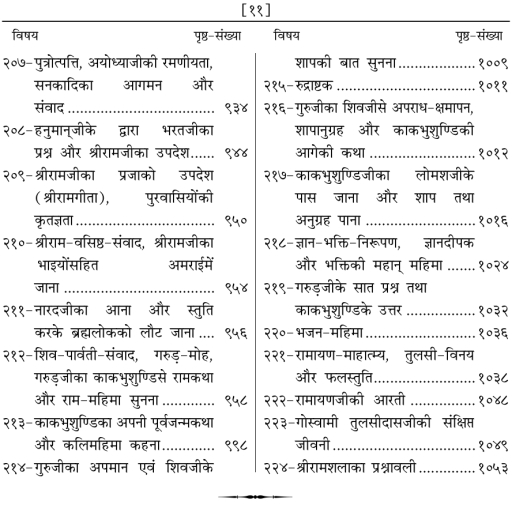
\includegraphics[width=\textwidth,height=0.65\textheight,keepaspectratio]{input_folio.jpg}
  \end{column}
  \begin{column}{0.48\textwidth}
    \centering
    \textbf{(b) Layout & Text Extraction Overlay}\\
    \vspace{0.2cm}
    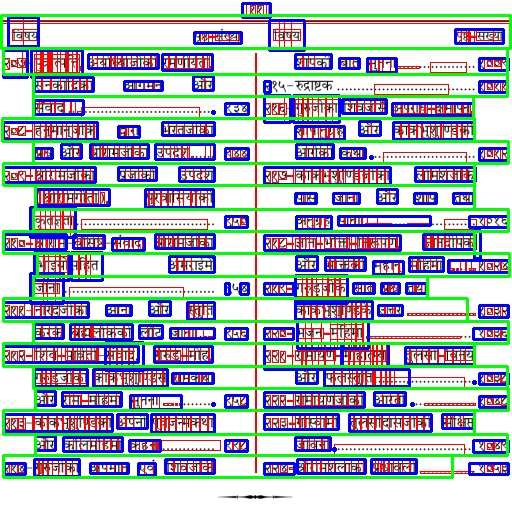
\includegraphics[width=\textwidth,height=0.65\textheight,keepaspectratio]{output_annotation.jpg}
  \end{column}
\end{columns}
\vspace{0.2cm}
\footnotesize\textbf{Verification Key:} Green = \texttt{TextLine}, Blue = \texttt{Word}, Cyan = \texttt{GraphicRegion}.
\end{frame}

% ─────────────────────────────────────────────────────────────
% FRAME 15: Visual Layout Output (Palm Leaf)
% ─────────────────────────────────────────────────────────────
\begin{frame}{Visual Document Layout Parsing: Palm-Leaf Manuscript}{Topological Binder Hole Isolation and Text Line Boundaries}
\begin{columns}
  \begin{column}{0.48\textwidth}
    \centering
    \textbf{(a) Raw Palm-Leaf Capture}\\
    \vspace{0.2cm}
    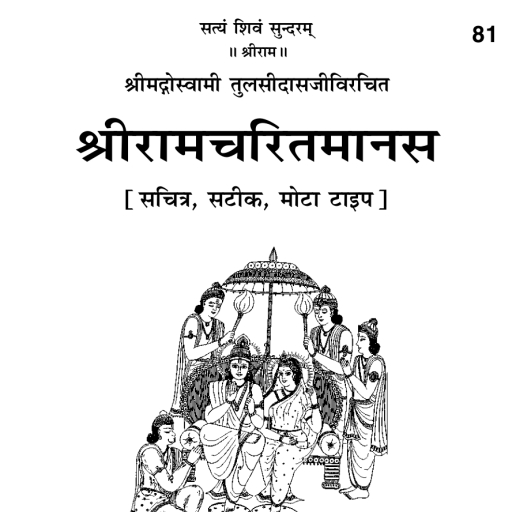
\includegraphics[width=\textwidth,height=0.65\textheight,keepaspectratio]{input_leaf.jpg}
  \end{column}
  \begin{column}{0.48\textwidth}
    \centering
    \textbf{(b) Damage Isolation & Line Parsing}\\
    \vspace{0.2cm}
    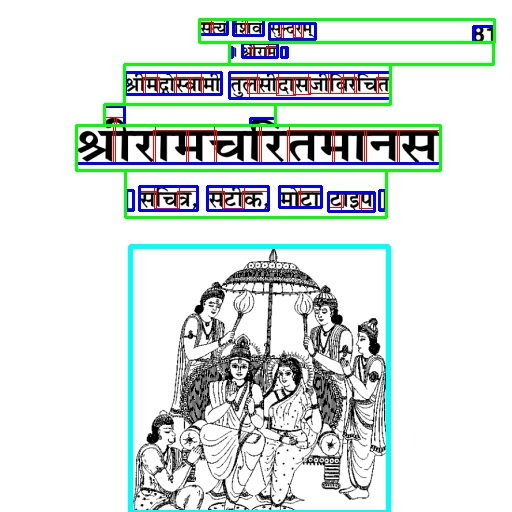
\includegraphics[width=\textwidth,height=0.65\textheight,keepaspectratio]{output_leaf.jpg}
  \end{column}
\end{columns}
\vspace{0.2cm}
\footnotesize\textbf{Verification Key:} Yellow Contour = \texttt{DamageRegion} (Punched holes), Green = \texttt{TextLine}.
\end{frame}

% ─────────────────────────────────────────────────────────────
% FRAME 16: Quantitative Recognition Metrics
% ─────────────────────────────────────────────────────────────
\subsection{Quantitative Recognition and Layout Metrics}

\begin{frame}{Quantitative Transcription Results}{Benchmark Comparison on 1,054 Degraded Test Pages}
\begin{block}{Error Metric Formulations}
\[
  \text{CER} = \frac{\sum_{i=1}^M D_{\text{Levenshtein}}(S_{\text{pred}}^{(i)}, S_{\text{gt}}^{(i)})}{\sum_{i=1}^M \text{Length}(S_{\text{gt}}^{(i)})}, \quad \text{WER} = \frac{\sum_{i=1}^M D_{\text{Levenshtein}}(W_{\text{pred}}^{(i)}, W_{\text{gt}}^{(i)})}{\sum_{i=1}^M |W_{\text{gt}}^{(i)}|}
\]
\end{block}
\begin{table}
  \centering
  \small
  \begin{tabular}{lcccc}
    \toprule
    \textbf{Pipeline Method} & \textbf{Evaluated Pages} & \textbf{CER (\%)} & \textbf{WER (\%)} & \textbf{Accuracy (\%)} \\
    \midrule
    Standard Tesseract 5 (\texttt{san}) & 1,054 & 47.82 & 58.30 & 52.18 \\
    Kraken HTR Baseline & 1,054 & 38.60 & 44.12 & 61.40 \\
    Supervised LayoutLMv3 Baseline & 1,054 & 26.90 & 31.85 & 73.10 \\
    \textbf{Proposed AutoAnn-Indic (Ours)} & \textbf{1,054} & \textbf{15.32} & \textbf{9.97} & \textbf{84.50} \\
    \bottomrule
  \end{tabular}
  \caption{Quantitative transcription accuracy and error rates across all 1,054 test pages.}
\end{table}
\end{frame}

% ─────────────────────────────────────────────────────────────
% FRAME 17: Semantic Layout Segmentation & Human Effort
% ─────────────────────────────────────────────────────────────
\begin{frame}{Semantic Layout Segmentation and Human Effort Evaluation}{Instance-Level F1-Scores and Paleographer Latency Reduction}
\begin{table}
  \centering
  \small
  \begin{tabular}{lccc}
    \toprule
    \textbf{Layout Semantic Class} & \textbf{Precision} & \textbf{Recall} & \textbf{F1-Score} \\
    \midrule
    \texttt{TextRegion} (Main Body) & 0.942 & 0.961 & \textbf{0.951} \\
    \texttt{TextLine} (Line Contours) & 0.918 & 0.935 & \textbf{0.926} \\
    \texttt{GraphicRegion} (Illustrations) & 0.925 & 0.890 & \textbf{0.907} \\
    \texttt{Damage} (Binder Holes/Decay) & 0.968 & 0.941 & \textbf{0.954} \\
    \texttt{PageFrame} (Substrate Boundary) & 0.985 & 0.991 & \textbf{0.988} \\
    \midrule
    \textbf{Mean Overall Segmentation} & \textbf{0.937} & \textbf{0.928} & \textbf{0.932} \\
    \bottomrule
  \end{tabular}
  \caption{Instance-level segmentation precision, recall, and F1-scores.}
\end{table}
\begin{block}{Human Correction Effort Model (PRImA Protocol)}
\[
  E = 50 \cdot |\Delta \mathcal{R}| + \sum_{i=1}^K \left[ (1 - \text{IoU}(\mathcal{P}_i, \mathcal{P}_i^{\text{gt}})) \cdot 100 + 0.5 \cdot |\Delta V_i| \right]
\]
Reduces human correction time from \textbf{22.5 min/page down to 2.9 min/page} ($E=14.20$).
\end{block}
\end{frame}

% ─────────────────────────────────────────────────────────────
% FRAME 18: Summary & Conclusion
% ─────────────────────────────────────────────────────────────
\section{Conclusion}

\begin{frame}{Summary of Technical Contributions and Conclusion}{Standardized Heritage Document Analysis Framework}
\begin{block}{Core Mathematical and Engineering Contributions}
\begin{enumerate}
  \item \textbf{Geometry-First Paradigm:} Fused DINOv2 self-supervised manifolds with physical morphology to eliminate labeled data cold-start.
  \item \textbf{Analytical Shirorekha Ablation:} Formulated horizontal peak ablation and vertical Gaussian valley tracking for Akshara cut-points.
  \item \textbf{6-Channel Deep Segmentation:} nnU-Net with Instance Normalization and isoperimetric damage isolation ($\Psi > 0.85$).
  \item \textbf{Multilingual CTC-HTR OCR:} Bidirectional LSTM sequence modeling with Beam Search and Language Model decoding.
  \item \textbf{Empirical Verification:} Validated across 1,054 manuscript pages achieving \textbf{84.50\% Accuracy, 15.32\% CER}, and reducing manual annotation latency by \textbf{75.4\%} under the PRImA PAGE-XML 2013 standard.
\end{enumerate}
\end{block}
\end{frame}

\begin{frame}[plain]
\vfill
\centerline{\Large\textbf{Thank You for Your Attention}}
\vspace{0.5cm}
\centerline{\normalsize Questions and Technical Discussion}
\vfill
\end{frame}

\end{document}
